\documentclass[12pt]{article}

\usepackage{graphicx}
\usepackage[hypertexnames=false,colorlinks=true,breaklinks]{hyperref}
\usepackage[dvipsnames]{xcolor}
\usepackage{amsmath}
\usepackage{amssymb}

\title{Tracking mice behavior in naturalistic settings with the Kalman filter
and smoother}

\author{}
\date{}

\begin{document}

\maketitle

\section{Introduction}

A central aim of current neuroscience is to understand the relation between
neural circuits and behavior. Many important behaviors are only observed in
naturalistic settings.  Therefore, signal processing methods to accurately
monitor behavior in these settings are essential.

Here we describe and evaluate the use of the Kalman Filter and Smoother to
perform inference in the Discrete Time Wiener Process Acceleration model, a
linear dynamical system model used for tracking. We use these inference methods
to track the position of mice while freely exploring a large arena.

\section{Methods}

\subsection{Mice foraging in naturalistic setting}

Videos were recorded of mice foraging in a circular arena (diameter two meters)
with two food patches (Figure~\ref{fig:foragingMouse}).

\begin{figure}
    \begin{center}
        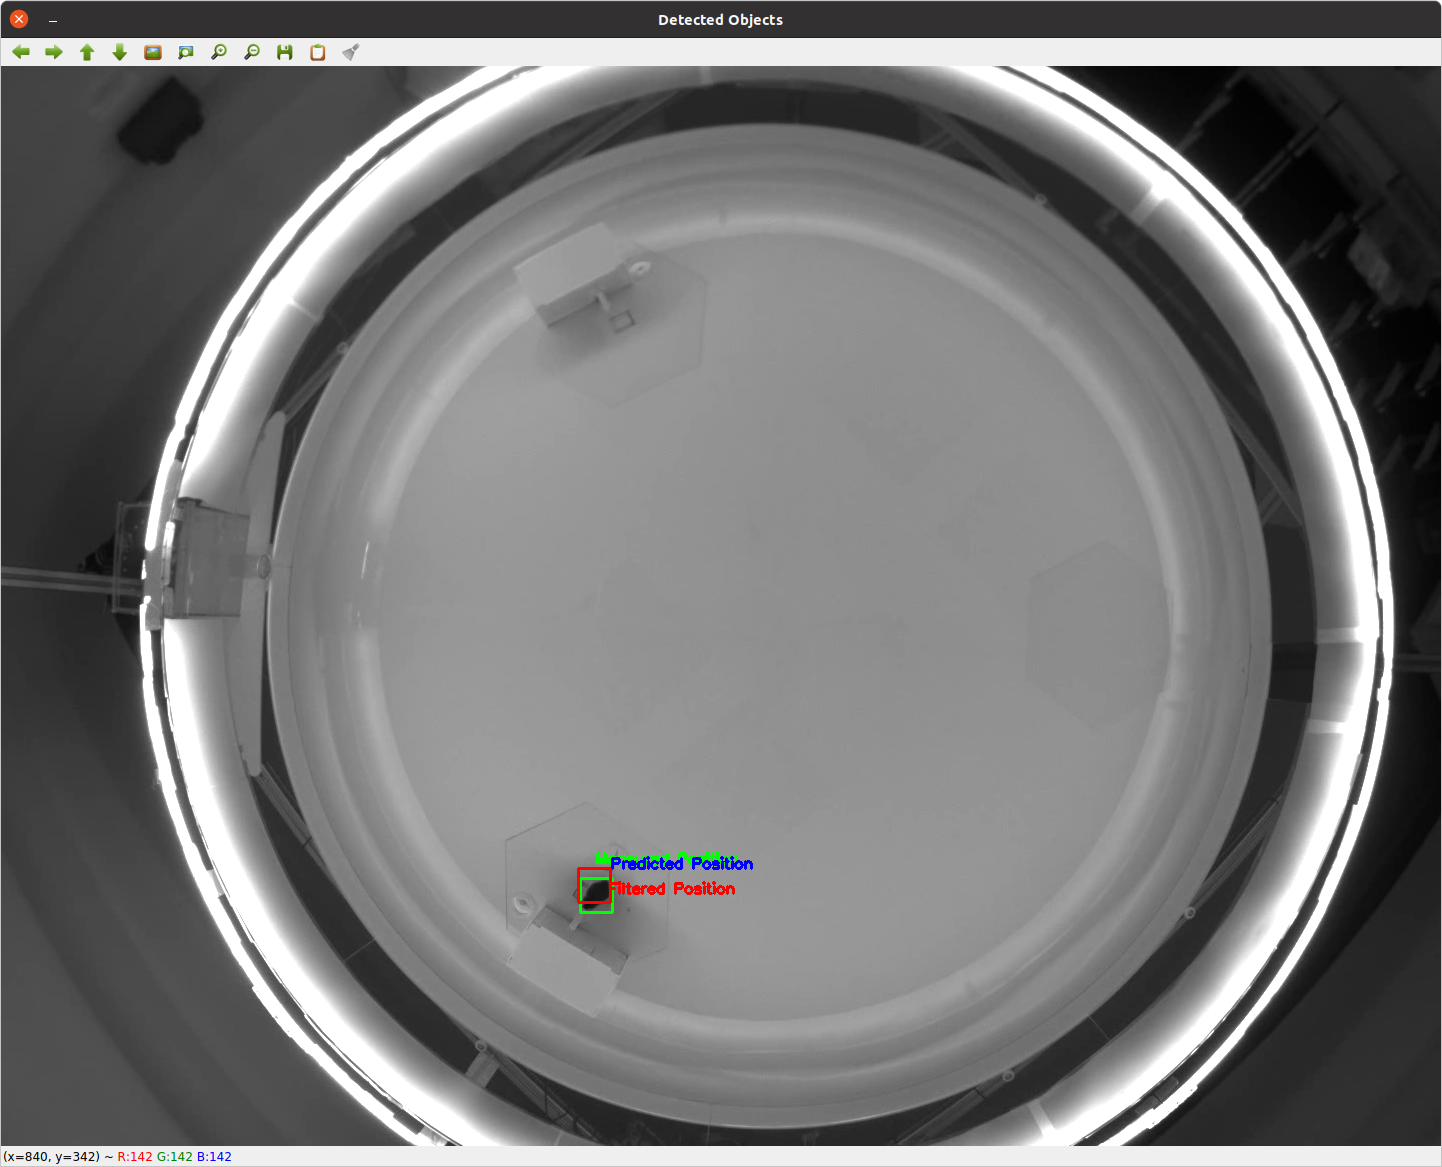
\includegraphics[width=4in]{figures/foraging.png}
        \caption{Video frame from a foraging mouse.}
        \label{fig:foragingMouse}
    \end{center}
\end{figure}

\subsection{Linear Dynamical System (LDS) model}

\textcolor{red}{You may want to fix the problem I marked in this section of
your poster.}

\subsection{Inference}

\subsubsection{Inference problems}

\textcolor{red}{Here I would insert the prediction, filtering and smoothing
equations.}

\subsubsection{Kalman filter}
\label{sec:kf}

\textcolor{red}{I would put the Kalman filter equations.}

\subsubsection{Kalman smoother}
\label{sec:ks}

\textcolor{red}{I would put the Kalman smoother equations. You may want to
comment that, as you will show in the results, the Kalman smoother yields more
accurate state estimates than the Kalman filter. However, the Kalman filter can
be used for online tracking, while the Kalman smoother cannot.}

\subsection{Discrete Wiener process acceleration (DWPA) model}
\label{sec:dwpaModel}
\begin{align*}
    \mathbf{x}_n&=[x_n,\dot{x}_n,\ddot{x}_n,y_n,\dot{y}_n,\ddot{y}_n]\\
    \mathbf{x}_n&=\begin{bmatrix}
        A & 0 \\
        0 & A
           \end{bmatrix}
           \mathbf{x}_{n-1}+\mathbf{w}_n,\quad\mathbf{w}_n\sim\mathcal{N}(\mathbf{0},Q),\quad Q=\begin{bmatrix}
                                                                                                    \textcolor{red}{\gamma_x^2}\tilde Q & \mathbf{0}\\
                                                                                                    \mathbf{0} &
                                                                                                    \textcolor{red}{\gamma_y^2}\tilde Q
                                                                                                \end{bmatrix}\\
    \mathbf{y}_n&=\begin{bmatrix}
        1 & 0 & 0 & 0 & 0 &0\\
        0 & 0 & 0 & 1 & 0 &0\\
           \end{bmatrix}
           \mathbf{x}_n+\mathbf{v}_n,\quad\mathbf{v}_n\sim\mathcal{N}(\mathbf{0},R),\quad R=\begin{bmatrix}
                                                                                               \textcolor{red}{\sigma_x^2} & 0\\
                                                                                                0 & \textcolor{red}{\sigma_y^2}
                                                                                            \end{bmatrix}\\
    \mathbf{x}_0&\sim\mathcal{N}(\textcolor{red}{\mathbf{m}_0},\textcolor{red}{V_0})
\end{align*}

\subsection{Computer vision functionality}
\label{sec:openCV}

We extracted the mouse position in each video frame using thresholding,
dilation, contour finding functions in the OpenCV library~\cite{c1}.

\subsection{Code availability}

Python code implementing the Kalman filter, Kalman filter and DWPA model can be
found at \cite{c2}.

\section{Results}

We first verified the accuracy of the DWPA model to estimate the position,
velocity and acceleration of a simulated mouse (Section~\ref{sec:simulatedMouse}). Then we used this model to
track the motion of a real mouse (Section~\ref{sec:realMouse}).

\subsection{Simulated mouse}
\label{sec:simulatedMouse}

We simulated the DWPA model with parameters $\mathbf{m}_0=[0, 0, 0, 0, 0,
0]^\intercal$, $V_0=\text{diag}(0.001)$, $\gamma_x=\gamma_y=1e4$ and
$\sigma_x=\sigma_y=100$ (Section~\ref{sec:dwpaModel}), generating samples of
true positions, velocities and accelerations (blue points in
Figures~\ref{fig:simulations_trueParams}a, b, c) and noisy measured positions (black
points in Figure~\ref{fig:simulations_trueParams}a). Note that the measured positions
contain a substantial amount of noise (compare the blue and black points in
Figure~\ref{fig:simulations_trueParams}).

We then run the Kalman filter (Section~\ref{sec:kf}, red traces in
Figures~\ref{fig:simulations_trueParams}a, b and c) and smoothing
(Section~\ref{sec:ks}, green traces in Figures~\ref{fig:simulations_trueParams}a, b and c).
Despite the large amount of noise in the simulations, the Kalman filter and
smoothing estimates were very accurate.
%
Position estimates were more accurate than velocity ones, which in turn were
more accurate than acceleration estimates.
%
As expected, smoothed estimates were more accurate than filtered ones for
positions, velocities and accelerations.

\begin{figure}
    \begin{center}

        \href{http://www.gatsby.ucl.ac.uk/~rapela/fwg/reports/learning/figures/46884517_pos_smoothed.html}{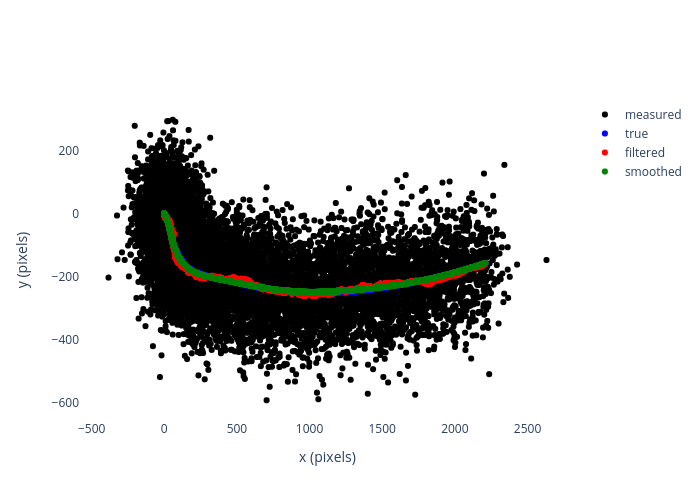
\includegraphics[width=3in]{figures/46884517_pos_smoothed.png}}
        \href{http://www.gatsby.ucl.ac.uk/~rapela/fwg/reports/learning/figures/46884517_vel_smoothed.html}{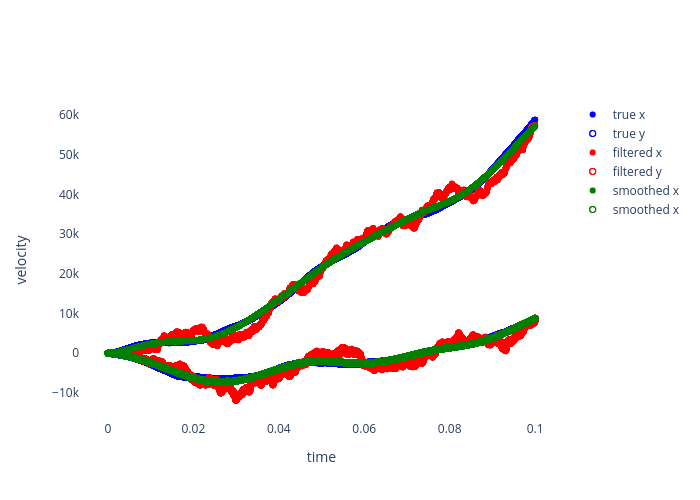
\includegraphics[width=3in]{figures/46884517_vel_smoothed.png}}
        \href{http://www.gatsby.ucl.ac.uk/~rapela/fwg/reports/learning/figures/46884517_acc_smoothed.html}{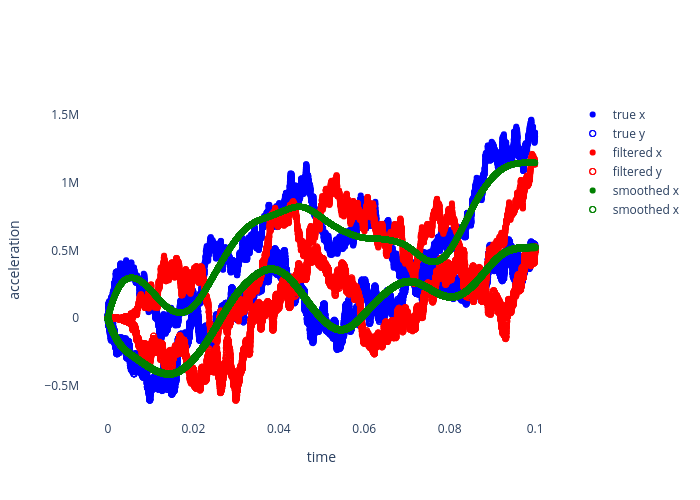
\includegraphics[width=3in]{figures/46884517_acc_smoothed.png}}

        \caption{Simulated mouse: filtered positions, velocities and accelerations using true parameters.}

        \label{fig:simulations_trueParams}

    \end{center}
\end{figure}

\subsection{Real mouse}
\label{sec:realMouse}

We first detected the horizontal and vertical positions of the mouse using the
computer vision functions described in Section~\ref{sec:openCV} (black points
of Figure~\ref{fig:realMouse}a). Note that when the mouse is behind the top
feeder, or entering the nest, black dots are missing, indicating that the
computer vision functions failed to detect the mouse position.

These missing positions are interpolated by the Kalman filter (red points in
Figure~\ref{fig:realMouse}a) and smoother (green points in
Figure~\ref{fig:realMouse}a). We observe that sometimes, the interpolations of
the Kalman filter are incorrect (e.g., missing observations next to the top
feeder). This problem is not present in Kalman smoother estimates (green points
in Figure~\ref{fig:realMouse}a).

Figures~\ref{fig:realMouse}b,c show velocity and acceleration estimates.
These estimates are reasonable. Velocities are at a minimum when the mouse is
near the patches or nest, and are at a maximum when the mouse is traveling
between patches. Accelerations are at a maximum when the mouse enters the arena
and when it leaves the food patches.

\begin{figure}
    \begin{center}

        \href{http://www.gatsby.ucl.ac.uk/~rapela/fwg/kf/postions_smoothed_session003_start0.00_end15548.27_startPosition1_numPosition10000.html}{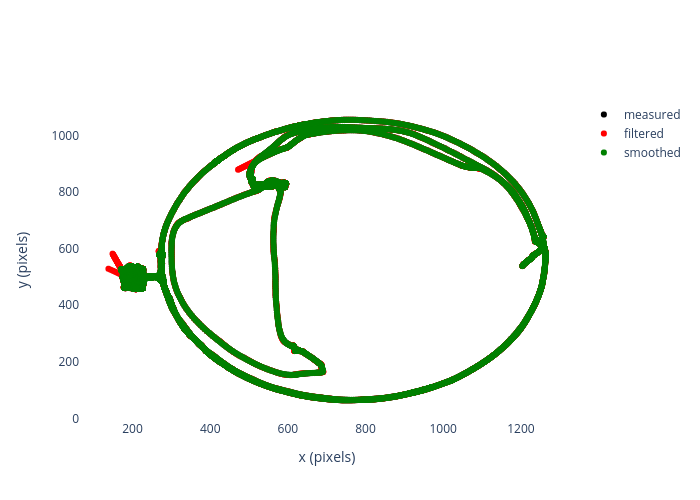
\includegraphics[width=3in]{{figures/positions_smoothed_session003_start0.00_end15548.27_startPosition1_numPosition10000}.png}}
        \href{http://www.gatsby.ucl.ac.uk/~rapela/fwg/kf/postions_velocities_session003_start0.00_end15548.27_startPosition1_numPosition10000.html}{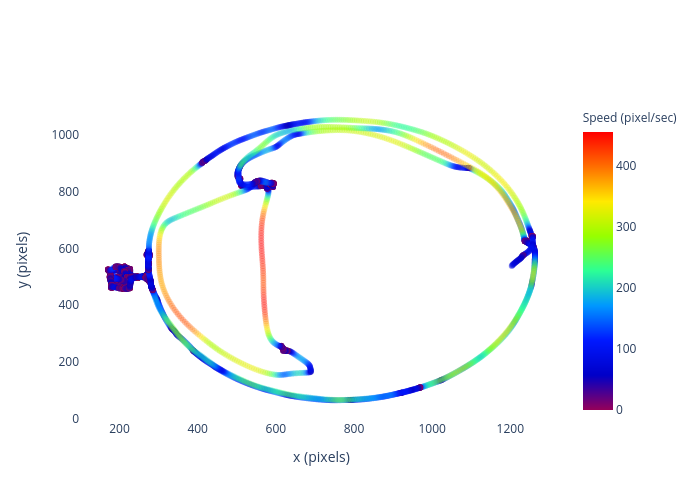
\includegraphics[width=3in]{{figures/positions_velocities_session003_start0.00_end15548.27_startPosition1_numPosition10000}.png}}
        \href{http://www.gatsby.ucl.ac.uk/~rapela/fwg/kf/postions_acelerations_session003_start0.00_end15548.27_startPosition1_numPosition10000.html}{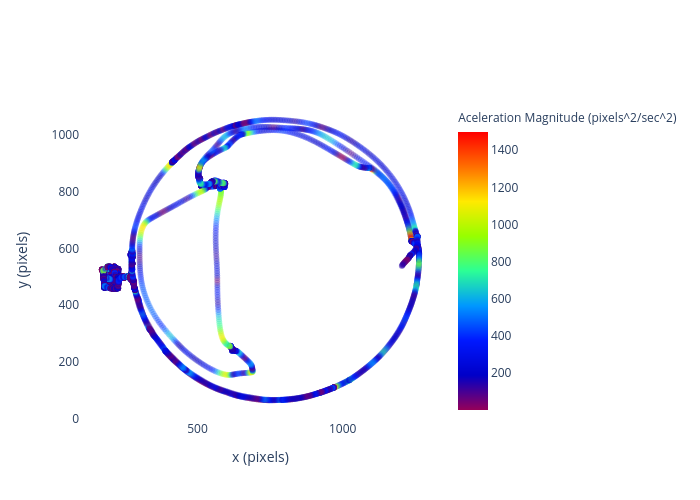
\includegraphics[width=3in]{{figures/positions_accelerations_session003_start0.00_end15548.27_startPosition1_numPosition10000}.png}}

        \caption{Real mouse: filtered positions, velocities and accelerations using true parameters.}

        \label{fig:realMouse}

    \end{center}
\end{figure}

\section{Ongoing work}

In this work we only discussed inference methods. That is, we assumed we knew
the model parameters and tried to infer the model states. However, in most
cases the model parameters are unknown and one needs to learn them from data.
In the last month of my fellowship I will study and apply learning techniques
for linear dynamical systems models. We plan to present our learning results
at~\cite{c3}.

\section{Summary}

In this project I \textbf{learned} an important time series model, the linear
dynamical systems model, as well as statistical methods to optimally infer the
model states, the Kalman filter and smoother. I studied the mathematical basis
of the inference methods and implemented them in Python.
%
I then used simulated data (for which I knew the true positions, velocities and
accelerations) to \textbf{evaluate the accuracy} of the Kalman filter and
smoother inferences.
%
Finally, I \textbf{applied} the above methods to estimate the position, velocity and
acceleration of \textbf{foraging mice}.

I feel fortunate to have learned a seminal model for time series data, and
associated inference methods, and to have applied them to understand an
important behavior.

\begin{thebibliography}{99}

\bibitem{c1} Bradski, G. (2000). The OpenCV Library. Dr. Dobb\&\#x27;s Journal of Software Tools.
\bibitem{c2} \url{https://github.com/Ash530888/Kalman-Smoother}
\bibitem{c3} A. Quershi, D. Campagner, M. Javadzadeh No, J. Rapela (submitted).  Tracking freely moving mice using computer vision, statistical inference and statistical learning techniques. 44th Annual International Conference of the IEEE Engineering in Medicine and Biology Society.  Glasgow, Scotland, UK. 2022.2022, 

\end{thebibliography}

\end{document}
